\section{Magnet}
The magnet bends charged particles moving inside and
outside of it. Lower the momentum of a particle, the more it is bent and vice
versa. The weight of the magnet is 12,000 tonnes, being the largest superconducting
magnet ever built.
\begin{figure}
  \begin{center}
  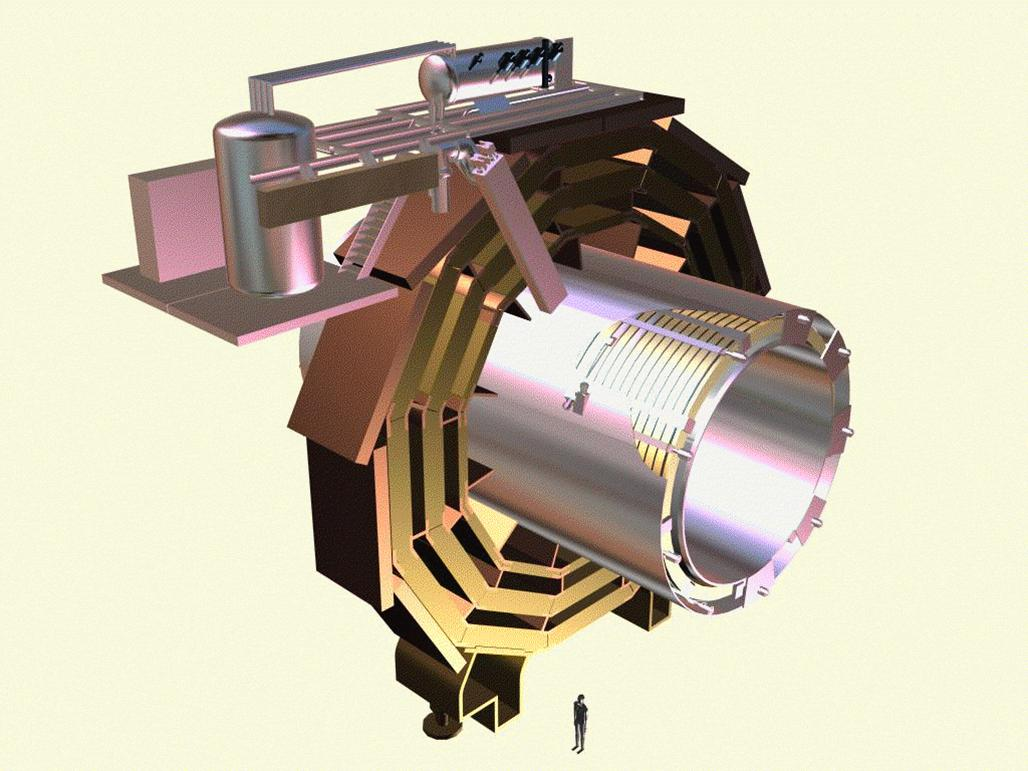
\includegraphics[width=0.50\linewidth]{Experiment/CMS/Image/cmssol.jpg}
	  \caption{An artistic view of the CMS solenoid~\cite{cmsSol}. 
	  An aluminum alloy shell, with a thickness of 50\unit{mm}, is placed on the 
	  inner and outer surface of the solenoid and used as a cooling wall.
	  Outside the solenoid are the return iron yokes which hold the 
	  magnetic flux.}
  \label{fig:cms_sol}
  \end{center}
\end{figure}
There are three main parts of the magnet: a solenoid, a vacuum 
tank, and the return iron yoke. A brief description of each component is given below:
\begin{itemize}[leftmargin=*]
\item \textbf{Solenoid}:
	The solenoid is made of NbTi (Niobium Titanium) coils which 
	is an aluminum-stabilized and mechanically reinforced superconducting 
	material. The solenoid is formed by placing 5 modules side-by-side 
	along the $z$-axis. With the length of 2.5\unit{m}, each module has 4 internal 
	layers of winding, each with 109 turns. Therefore, the total length of 
	the solenoid is $5\times 2.5$\unit{m} $ = 12.5$\unit{m}, with $5\times 4 \times 109 = 
	2180$ turns. The diameter of the solenoid is 6\unit{m}. The magnetic field 
	inside the solenoid is given by
	\begin{equation}
		B = k\mu_0\times N\times I/L
	\end{equation}
	Where $k$ is the relative permeability. Therefore, with 
	\textit{k} = 0.90, $\mu_0 = 4\pi\times 10^{-7}$\unit{mT/A}, N = 2180, 
	I = 19.14\unit{kA}, and L = 12.5\unit{m}, the magnetic field inside the solenoid, 
	B = 3.8\unit{T}, which is 100,000 times stronger than the Earth's magnetic 
	field. Being a very high energy experiment, such a large magnetic 
	field is necessary for better tracking resolution.
\item \textbf{Vacuum tank}: A huge amount of heat is produced due to the 
	flow of such a large current. The energy contained inside the solenoid 
	is 2.7\unit{GJ} which is more than enough to melt 18 tonnes of gold. A 
	dedicated cooling system is placed to cool the solenoid down to 
	-268$^\circ$C.
\item \textbf{Return yoke}: With four layers in the barrel region, and six
	disks in the endcap region, a giant iron return yoke is placed outside 
	the solenoid to contain the magnetic flux. The iron yokes in the barrel 
	region are shown in Figure~\ref{fig:cms_sol}. Total weight of the
	iron yoke is 10000 tonnes.
\end{itemize}

The longitudinal and transverse component of the magnetic field produced from 
the solenoid is shown in Figure~\ref{fig:cms_mag}. The longitudinal component
is the strongest compared to the transverse component. The transverse one
 is everywhere zero except at the endcap in the region 6\unit{m} $<z<$ 10\unit{m}. 
The magnetic field of the longitudinal component is 3.8\unit{T} inside the solenoid,
and about 2\unit{T} inside the return iron yoke. Further, the longitudinal component
inside and outside the solenoid is in the opposite direction. By virtue of this property, 
the charged particles are bent in the opposite direction.
\begin{figure}
  \centering
  \subfigure[Longitudinal component of the magnetic field
  \label{subfig:cms_magl}]
  {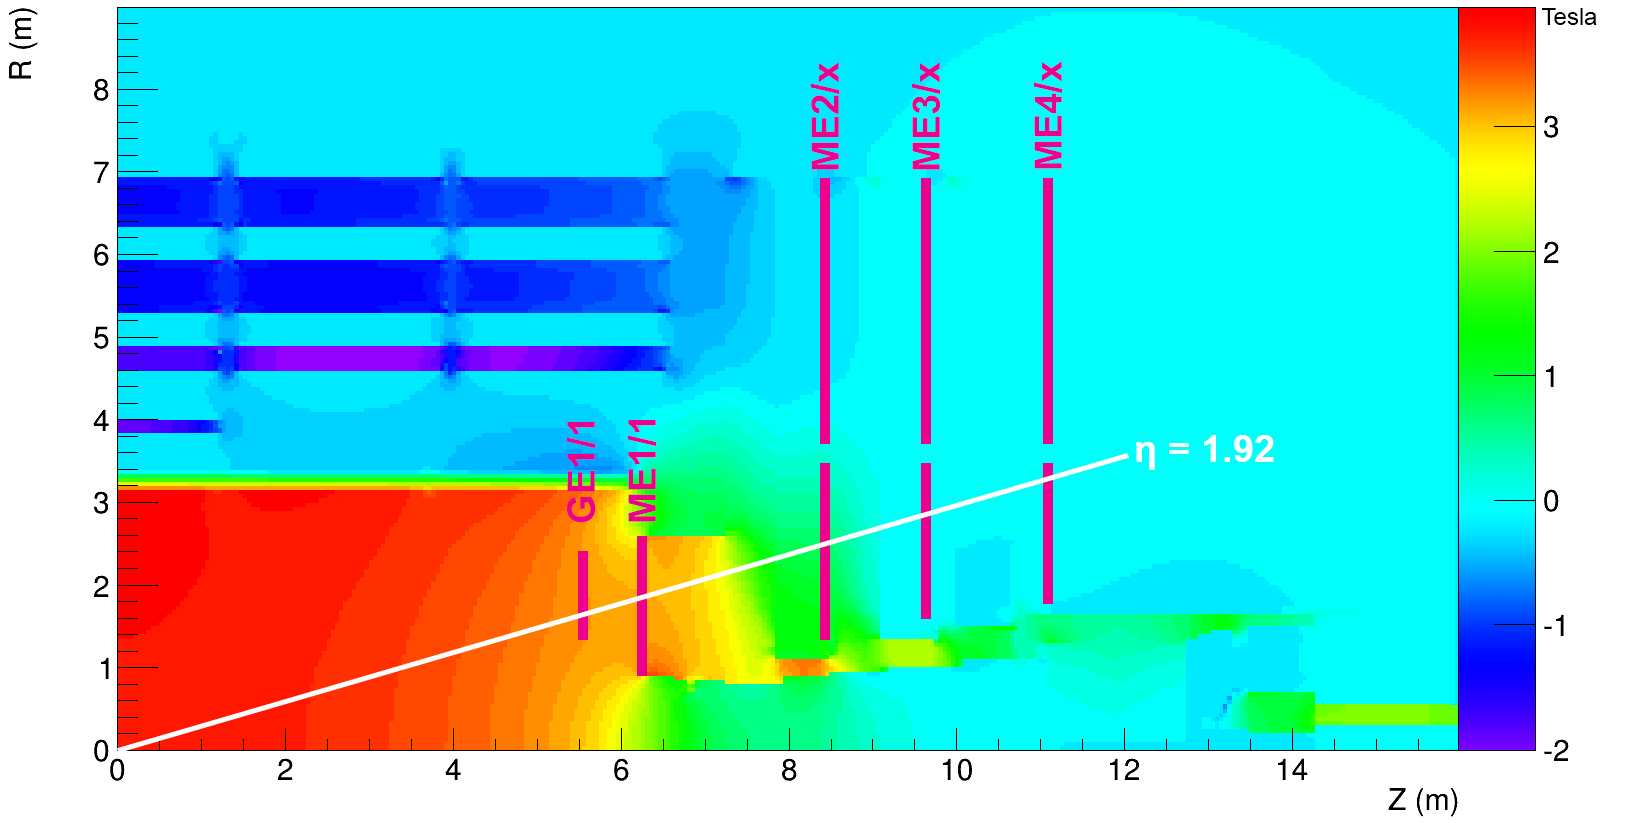
\includegraphics[width=0.50\linewidth]{Experiment/CMS/Image/magl.png}}
  \hfil
  \subfigure[Transverse component of the magnetic field
  \label{subfig:sinti_magt}]
  {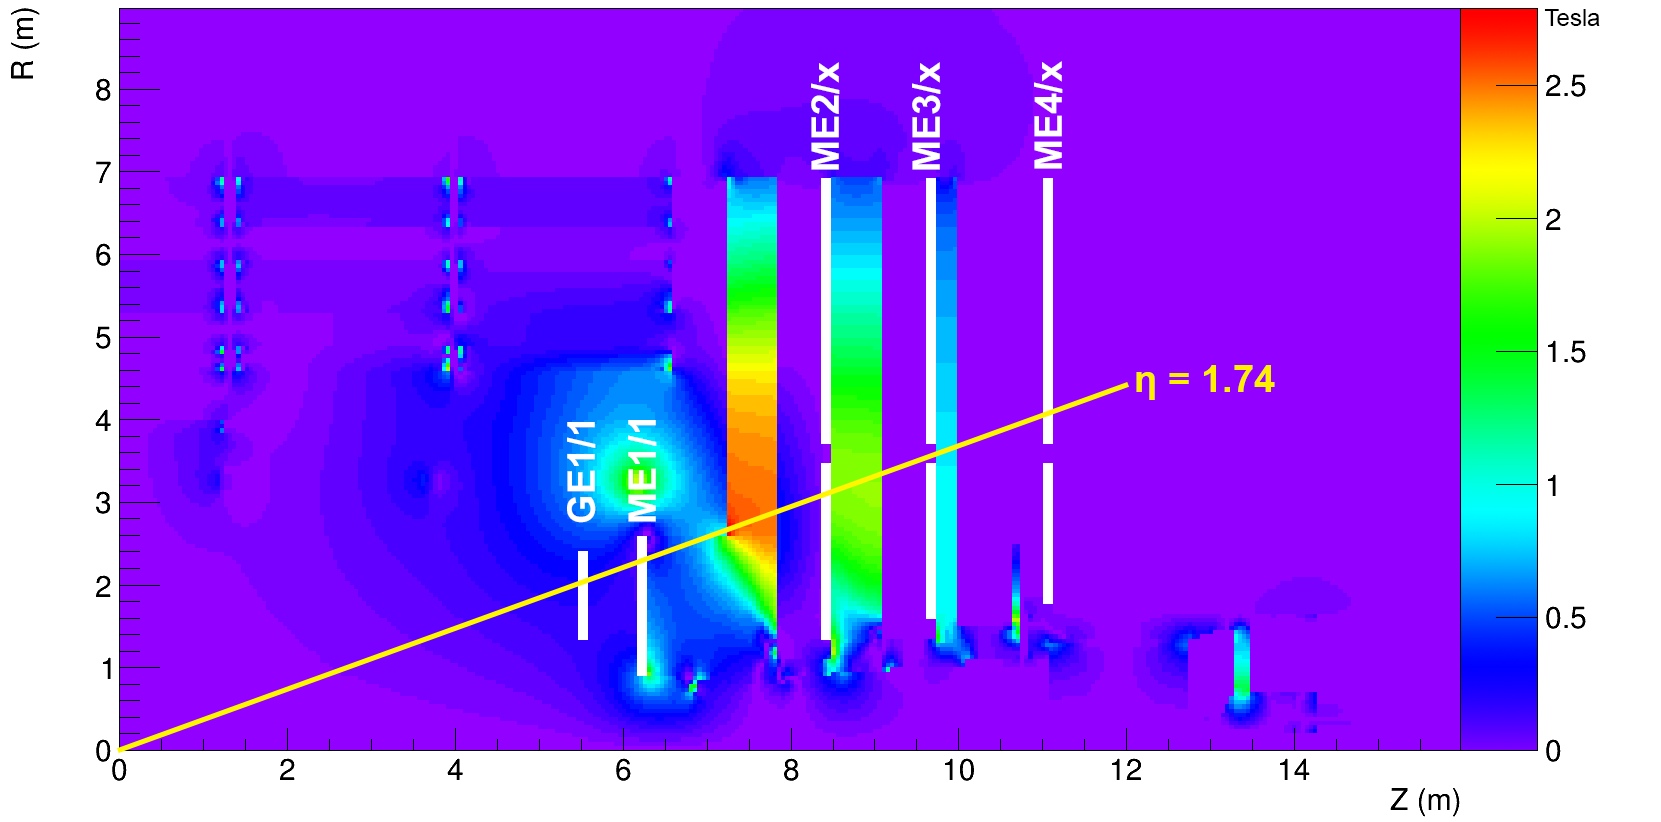
\includegraphics[width=0.50\linewidth]{Experiment/CMS/Image/magt.png}}
	\caption{Component of the magnetic field inside CMS~\cite{Lenzi:2013xpa}.}
  \label{fig:cms_mag}
\end{figure}

